\subsection{Иерархическая кластеризация}
\subsubsection{Идея метода}

Мы все из биологии помним, что всё живое на земле делится на следующую иерархию: царство, порядок, семейство, род, вид и так далее. Каждая из ступенек этой иерархии является непересекающейся группой, которую мы и будем называть кластером.

{\bf Суть} иерархической кластеризации заключается в том, чтобы взять и разделить весь наш {\it input space} (входное пространство) на части, но только не плоско, а, грубо говоря, вложено. То есть снача мы делим на несколько частей, каждая из которых делится ещё и ещё до тех пор, пока результат нас не устроит. 

Есть 2 достаточно очевидных, но принципиально разных способа реализации данного алгоритма "--- {\it Agglomerative} (восходящие) и {\it Divisive} (нисходящие).

Визуализация данных, как правило, осуществляется с помощью {\bf дендрограммы} (дерево, то есть граф без циклов).

\subsubsection{Agglomerative}
Наиболее подходит для случая, когда нам нужно получить большое количество кластеров.
Так же данный вариант обычно немножко проще реализуется.
\begin{enumerate}
\item начинаем с ситуации, когда каждый объект – отдельный кластер;
\item на каждом шаге совмещаем два наиболее близких кластера, получая из них один новый;
\item останавливаемся, когда получаем требуемое количество или единственный кластер.
\end{enumerate}

\begin{figure}[H]
\centering
    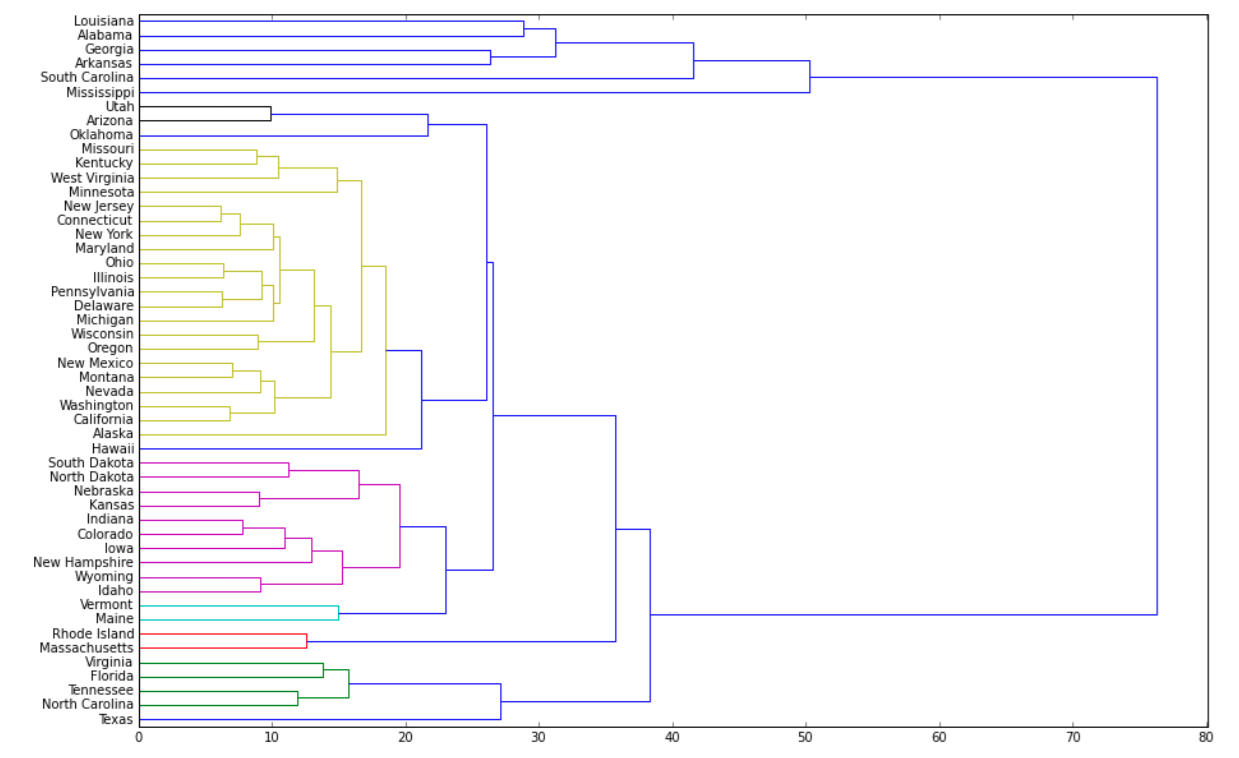
\includegraphics[width=150mm]{images/agl.png}
    \caption{Пример дендограммы восходящей кластеризации на основе красно-синих штатов.}
    \label{alg}
\end{figure}

\subsubsection{Divisive}
Более удобен, когда нам нужно несколько кластеров.
\begin{enumerate}
\item начинаем с ситуации, когда все объекты составляют один большой кластер;
\item на каждом шаге разделяем каждый кластер две или несколько частей;
\item останавливаемся, когда получаем требуемое количество или заранее заданное $N$ кластеров.
\end{enumerate}

\begin{figure}[H]
\centering
    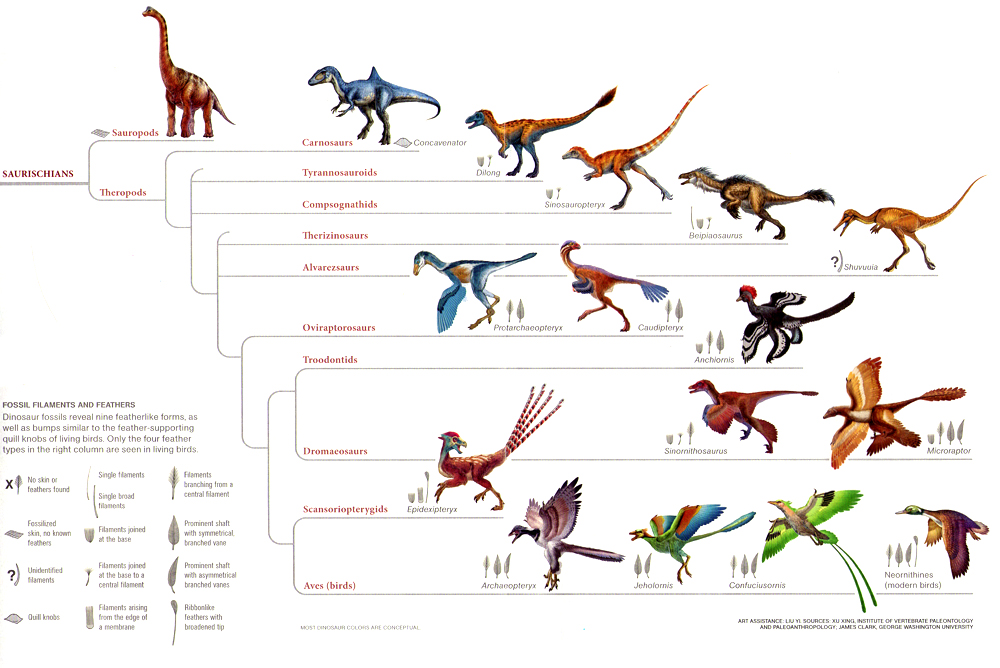
\includegraphics[width=150mm]{images/dino.jpg}
    \caption{Пример дендограммы нисходящей кластеризации на основе классификации динозавров.}
    \label{dino}
\end{figure}


\subsubsection{Реализация алгоритма}
Рассмотрим восходящий алгоритм в виде псевдокода на языке $Python$:
\begin{lstlisting}
function agglomerative(X, K):
    initialize N # number of objects 
    initialize C = N # number of clusters initialize 
    C_i = x_i # initial clusters 
    while C>K:
        C_a = C_b = None # closest clusters 
        min_dist = +inf # distance between closest 
        for i in 1 .. C:
            for j in i + 1 .. C:
                dist = d(C_i, C_j) # dist. betw. clusters 
                if dist < min_dist:
                    min_dist = dist 
                    C_a = C_i 
                    C_b = C_j
        merge(C_a, C_b)
        C=C - 1
    return C_1, ... , C_k
\end{lstlisting}

Как мы видим, необходимая память $O(N^2)$, а вычислительная сложность данного алгоритма $О(N^2 \log N)$ (хорошо, что не куб). Получается, что этот алгоритм вычислительно очень дорогой и применять его на очень больших объемах данных очень непродуктивно, и никакой памяти не хватит. Но у него есть несколько приемуществ: удобная визуализация и не сложно выбрать количество кластеров.

\subsubsection{Stepwise-optimal HC}
Что плохого в том алгоритме, что мы описали выше?

На каждом шаге мы пытаемся совместить два кластера, но не очень понимаем почему и зачем. Понятно, что минимальное расстояние между класстерами -- это хорошо. Придумали сделать некое обобщение этого алгоритма, который позволяет делать всё тоже самое для произвольного критерия качества ($J$).

Окаывается, что те расстояния между кластерами, которые мы использовали, имеют под собой функционал, который они оптимизируют. В частности 
$d_{max}$ обеспечивает наименьшее увеличение диаметра кластера.
Так же часто используется расстояние
$d_e$ (см.~\ref{de}), которое обеспечивает наименьшее увеличение квадратичного критерия (квадратичный критерий "--- это сумма расстояний внутри кластера от каждого объекта, до соответствующего центра).

\begin{equation}\label{de}
d_e(C_i,C_j) = \sqrt{\frac{n_i n_j}{n_i+n_j}}||m_i - m_j||
\end{equation}

Рассмотрим данный алгоритм в виде псевдокода на языке $Python$:
\begin{lstlisting}
function swo(X, K):
    initialize N # number of objects
    initialize C = N # number of clusters initialize 
    C_i = x_i # initial clusters 
    while C > K:
        # choose the pair that optimizes
        # the given criterion J when merged
        C_a, C_b = find_best_merge(J, C_1, ..., C_C) 
        merge(C_a, C_b)
        C=C - 1
    return C_1, ... , C_k
\end{lstlisting}

\subsubsection{Неевклидовы пространства}

{\it Как измерить расстояние между кластерами, если невозможно определить центроид?}

Оказывается, что иерархический подход так же работает, но только нужно изменить функцию растояния между кластерами.

{\bf Идея.} В каждом из кластеров выбрать <<типичныи представителя>> "–-- clustroid. Считать расстояние не между кластерами, а между <<кластроидами>>

Каким образом выбрать <<типичного представителя>> ?

Есть несколько подходов. 
Можно выбать такой объект, для которого
\begin{itemize}
\item минимальная сумма расстояний до других объектов в кластере (он находится в центре);
\item сумма квадратов расстояний до других объектов в кластере минимальна; 
\item максимальное расстояние до других объектов в кластере минимально.
\end{itemize}

Таким образом можно кластеризовать что-то другое помимо числовых векторов.

\subsubsection{Плюсы и минусы алгоритма}
\begin{itemize}
\item[+] Могут получиться несферические кластеры;
\item[+] Можно придумать разнообразие критерии, как разнообразные виды расстояния между кластерами, так и между объектами;
\item[+] Поддерживает любые $K$ из коробки (то есть один раз запустив алгоритм, мы уже кластеризовали наши объекты на любое количество кластеров);
\item[-] Требует много вычислительных ресурсов, невозможно работать при больших объёмов данных.
\end{itemize}

\subsection{<<Быстрая>> модификация алгоритма}
\begin{lstlisting}
function fast_agglomerative(X, K):
    initialize N # number of objects
    initialize C = N # number of clusters initialize 
    C_i = x_i # initial clusters initialize 
    delta_set = get_delta_set(C_i) 
    while C > K:
        C_a = C_b = None # closest clusters 
        min_dist = +inf # distance between closest 
        for C_i in delta_set:
            for C_j in delta_set:
                dist = d(C_i, C_j) # dist. betw. clusters 
                if dist < min_dist:
                    min_dist = dist
                    C_a = C_i; C_b = C_j 
        new_cluster = merge(C_a, C_b)
        update_delta_set(C_i, new_cluster) 
        C = C - 1
        if delta_set is empty:
            delta_set = get_delta_set(C_i) 
    return C_1, ..., C_K
\end{lstlisting}

{\it Осталось только понять, что же такое этот delta-set и откуда его брать.}

{\bf Delta-set} --– набор кластеров расстояние между которыми меньше $\delta$. Чтобы реализовать функцию {\bf get-delta-set} нужно учитывать следующие моменты:
\begin{enumerate}
\item Если $C \le K_1$, то $\delta$-set – это все $C_i$;
\item Иначе выбрать $K_2$ случайных расстояний между кластерами, $\delta = \min{K_1,K_2}$;
\item $K_1$ и $K_2$ влияют только на скорость, но не на результат кластеризации; 
\item рекомендованные значения $K_1 = K_2 = 20$.
\end{enumerate}